% !TEX root = ../thesis.tex

\chapter{Case Study I: Building Health Monitoring} \label{chp:building}

\section{Domain and Experimental Objectives}

In the contemporary Architecture, Engineering, and Construction (AEC) domain, digital transformation has evolved from a forward-looking concept to an indispensable strategic imperative. Its core driving force stems from the urgent need for efficient, precise, and sustainable management of physical infrastructure throughout its entire lifecycle \cite{boje2020towards, lu2020digital}. With the increasing maturity of sensor technology, laser scanning, photogrammetry, and Building Information Modeling (BIM), we are capturing and storing massive amounts of data about the built environment with unprecedented capability \cite{tang2019retrieving, li2024single}. This trend has given birth to Digital Twins as a core technological paradigm, promising to revolutionize how we understand, monitor, and maintain complex building systems by constructing dynamic, high-fidelity virtual replicas of physical assets \cite{tao2018digital}.

\begin{figure}[htbp]
\centering
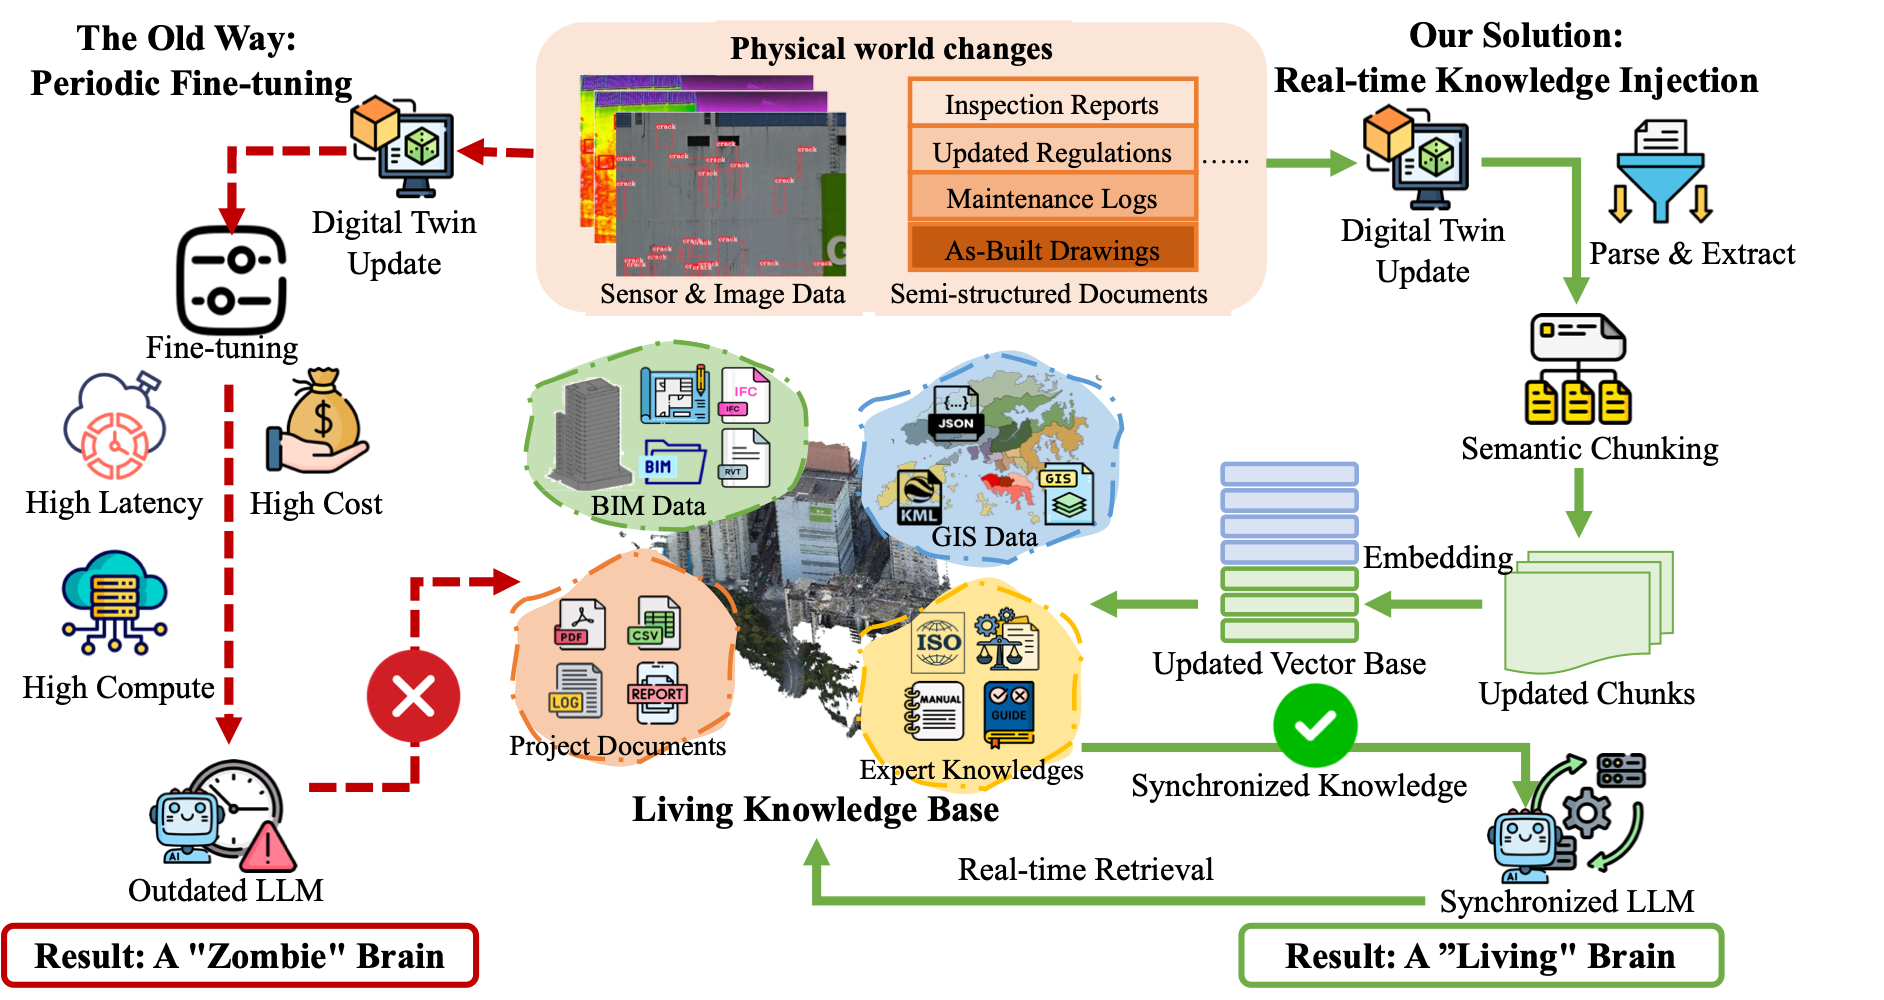
\includegraphics[width=0.9\textwidth]{figures/DefectGPT/dynamic_knowledge_engine.png}
\caption{Dynamic Knowledge Engine: Comparison between traditional periodic fine-tuning approach (left) resulting in a "Zombie Brain" versus our real-time knowledge injection solution (right) creating a "Living Brain" that continuously updates with physical world changes.}
\label{fig:dynamic-knowledge-engine}
\end{figure}

Theoretically, a well-developed Digital Twin should integrate all information from geometric morphology and material properties to real-time operational states, thereby providing decision-makers with an omniscient "God's eye view" perspective. However, in practical exploration, we have discovered that current mainstream Digital Twin applications remain largely at the level of "data representation" \cite{negri2017review}. They excel at answering descriptive questions such as "what" and "where," for example, precisely locating a specific structural component or a detected surface defect within a three-dimensional model. This undoubtedly represents a tremendous leap forward compared to traditional management modes based on drawings and documents, effectively solving the long-standing "data silo" problem in the industry \cite{bruno2018historic}.

However, when decision-making requirements escalate from simple information retrieval to complex causal analysis and diagnostic reasoning, the fundamental limitations of existing Digital Twin paradigms become starkly apparent. The real challenges faced by engineers and managers are not merely knowing that defects exist, but deeply understanding "why" certain patterns of defects occur and assessing potential risks based on this understanding \cite{hamdan2021semantic}. Answering such questions requires systems to possess capabilities beyond data representation—namely, "cognitive reasoning" capabilities. This demands that systems not only access data but understand the domain knowledge, physical laws, and engineering logic embedded within the data.

\subsection{Critical Flaws in Direct LLM Application}

With the rise of Large Language Models (LLMs), an seemingly obvious solution emerges: utilizing their powerful natural language understanding and generation capabilities to serve as a "bridge" across this gap. Initial attempts show that LLMs can indeed parse natural language queries and understand document content to some extent. However, through in-depth research, we have discovered that this direct, naive application approach constructs an extremely dangerous "unstable bridge" with three fatal, interconnected structural flaws \cite{ji2023survey}.

First is the inherent limitation of context windows. LLMs are strictly constrained by their context length when processing information, like observing a complex building system through a narrow keyhole. For diagnostic tasks requiring integration of multiple large documents, maintenance records spanning several years, and massive sensor data, this "tunnel vision" information processing approach inevitably leads to missing critical information and misjudging the overall situation \cite{liu2023lost}.

Second is the lack of domain-specific grounding. While general-purpose LLMs are knowledgeable, their knowledge is generalized and statistical, lacking deep understanding of physical laws and causal relationships specific to engineering domains. Their knowledge is like a "floating anchor" that cannot firmly connect with the seabed, unable to establish stable connections with highly specialized domain knowledge in building diagnosis, causing reasoning processes to deviate from basic engineering principles \cite{harnad1990symbol}.

Third, and most dangerously, is factual hallucination and inaccuracy. Due to the combined effect of the above two flaws, LLMs are prone to generating seemingly reasonable but completely factually incorrect "hallucination" outputs when faced with queries beyond their knowledge boundaries or with insufficient information. While this might be tolerable in entertainment or general Q\&A scenarios, in engineering decisions concerning structural safety and public interest, any conclusion based on hallucination could lead to catastrophic consequences \cite{zhang2023siren}.

\subsection{Research Objectives}

Therefore, this chapter's core research task is not simply applying LLMs to building diagnosis, but fundamentally redesigning information processing and reasoning architecture to construct a truly stable, reliable, and intelligent "cognitive bridge." We aim to answer the core question: How can we design and implement an intelligent agent architecture that safely and efficiently integrates multimodal Digital Twin data with deep domain knowledge, thereby endowing systems with genuine diagnostic reasoning capabilities?

To answer this question, we propose a concrete implementation based on the CORTEX theoretical framework—DefectGPT. This chapter will elaborate on DefectGPT's design philosophy, system architecture, and implementation details, and through rigorous controlled experiments, quantitatively evaluate its performance gains relative to current optimal methods, thereby providing solid empirical support for RQ1 and RQ3.

\section{Twin Construction and CORTEX Implementation}

To systematically address the aforementioned "reasoning gap" problem, we design and implement a CORTEX intelligent agent customized for building defect diagnosis tasks—DefectGPT. Its core design philosophy lies in repositioning the role of Large Language Models (LLMs): rather than viewing them as omniscient, centrally-located "brains," we position them as powerful, controlled "reasoning interfaces." This interface does not possess ultimate domain truth but is mandatorily required to think and express based on a rigorously validated knowledge base that maintains real-time synchronization with the physical world.

\subsection{Building Diagnosis Task Formalization}

We define building asset diagnosis tasks as a heterogeneous data-based Question Answering (QA) problem with the following formal specification:

\textbf{Input}: Natural language question $Q$ expressing diagnostic intent\\
\textbf{Knowledge Source}: An L1 descriptive twin $\mathcal{DT}_{L1}$ containing multimodal building data\\
\textbf{Output}: An evidence-based, traceable answer $A$ with source attribution

The L1 descriptive twin $\mathcal{DT}_{L1}$ is formally defined as:
\begin{equation}
\mathcal{DT}_{L1} = \{S, D, K\}
\end{equation}
where $S$ represents spatial information carriers, $D$ represents defect data schemas, and $K$ represents domain knowledge repositories.

\subsection{L1 Descriptive Twin Construction}

Following the three-tier framework established in Chapter 3, we construct a comprehensive L1 descriptive twin through a layered approach that transforms raw, chaotic physical world information into structured, machine-queryable knowledge assets.

\begin{figure}[htbp]
\centering
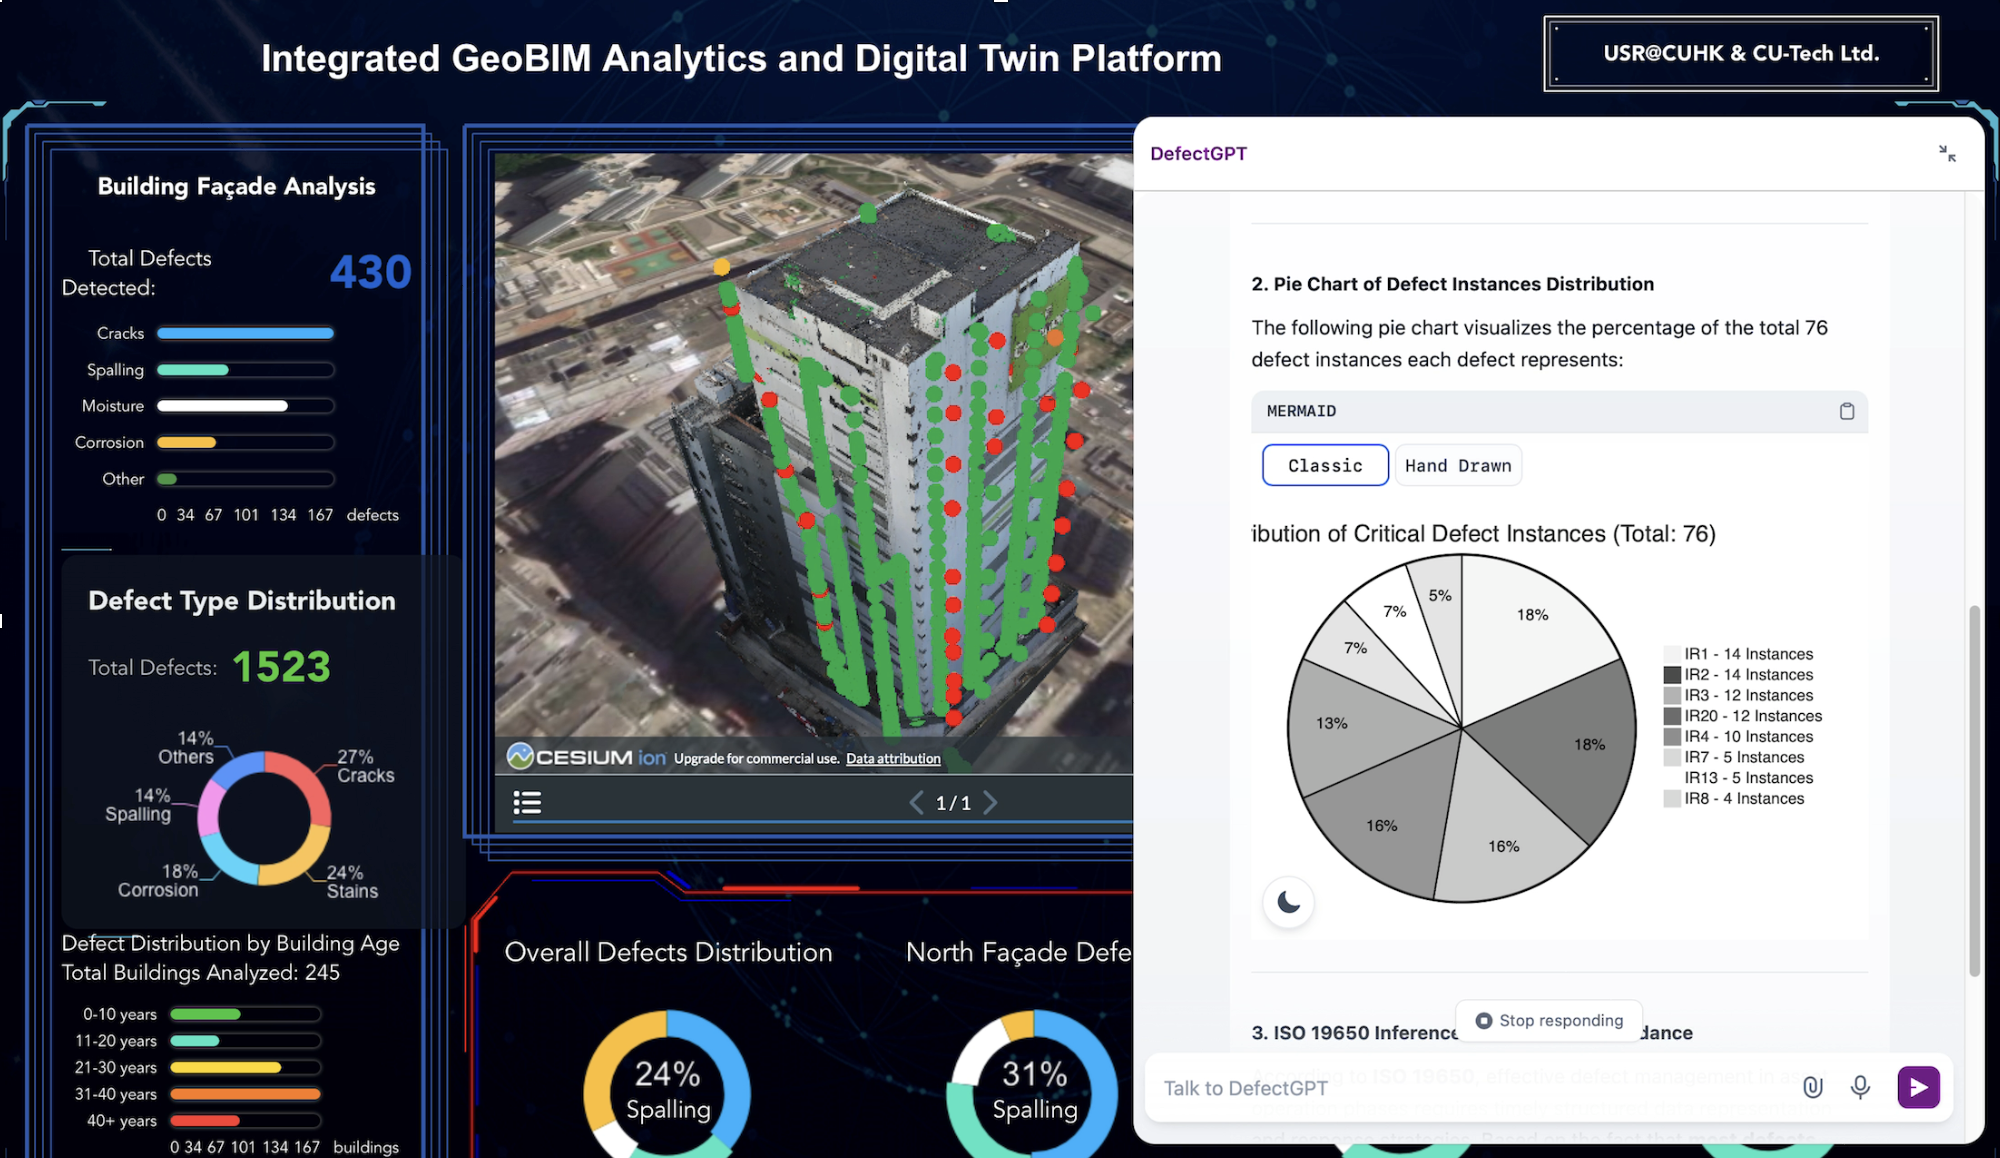
\includegraphics[width=0.9\textwidth]{figures/DefectGPT/System_implement.png}
\caption{Comprehensive System Implementation Architecture showing the three-layer Digital Twin structure: Data Layer (GeoBIM modeling, defect modeling, expert knowledge), Digital Twin Layer (spatial information carriers, defect data schemas, domain knowledge repository), and Decision Layer (hybrid retrieval and cognitive reasoning).}
\label{fig:system-implementation}
\end{figure}

\textbf{Data Layer: Multi-Modal Information Processing}: The Data Layer serves as the perceptual foundation of the entire system, with its core responsibility being comprehensive ingestion of all raw information related to building assets from diverse physical and digital sources. The challenge lies not only in the massive volume of data but also in the diversity of sources, heterogeneity of formats, and complexity of semantics.

\textbf{GeoBIM Modeling}: This module processes core spatial and geometric information of buildings, representing a deep fusion of traditional BIM with Geographic Information Systems (GIS). BIM provides microscopic information about building interiors, such as precise three-dimensional geometry, material properties, topological relationships, and functional definitions of individual components (beams, columns, walls). GIS provides macroscopic environmental information about buildings, including geographic coordinates, surrounding environment, orientation, sunlight conditions, and connections to municipal infrastructure \cite{boje2020towards}.

\textbf{Defect Information Modeling}: This module focuses on objective, quantitative characterization of building physical defects. We employ an automated detection workflow based on multi-sensor fusion. Using UAVs equipped with high-definition visible light cameras and infrared thermal imaging, we systematically scan building facades through photogrammetry and structured light techniques to generate high-resolution three-dimensional point clouds and texture models. Subsequently, deep learning computer vision algorithms (such as Convolutional Neural Networks) analyze image and point cloud data to automatically detect, segment, and locate various types of defects including cracks, spalling, water seepage, and delamination \cite{spencer2019advances}.

\textbf{Expert Knowledge Collation}: This serves as the bridge connecting observational data with diagnostic conclusions. The module systematically collects, organizes, and digitalizes all text and semi-structured knowledge related to building diagnosis, including national and local technical standards and legal regulations defining mandatory requirements and safety benchmarks for defect assessment; design drawings and as-built documentation recording original design intent and actual construction conditions; historical maintenance and inspection reports describing numerous historical problems and treatment measures in natural language; and professional manuals and diagnostic guides written by senior engineers containing substantial experience-based heuristic knowledge \cite{hamdan2021semantic}.

\textbf{Digital Twin Layer: Knowledge Organization}: The Digital Twin Layer serves as the "organizer" and "refiner" of knowledge, with its core task being transformation of raw, chaotic information ingested by the Data Layer into machine-readable, computable, and reasoning-capable, highly structured and interoperable knowledge assets.

\textbf{Spatial Information Carriers}: Raw model data from the GeoBIM module is parsed and standardized here. We adopt open standards such as Industry Foundation Classes (IFC) and CityGML to transform BIM and GIS models generated by different software into unified, semantically rich formats. This process ensures that definitions of components like "beams" or "walls" are consistent and machine-understandable throughout the system \cite{tang2019retrieving}.

\textbf{Structured Defect Data Schemas}: Detection results from the defect modeling module are rigorously structured here. We design a unified defect data schema storing complete properties of each defect in JSON or CSV formats. This schema includes not only geometric and type information but also timestamps, associated sensor readings, corresponding BIM component IDs, and links to original image evidence \cite{li2024single}.

\textbf{Domain Knowledge Repository}: This handles expert knowledge processing. All unstructured and semi-structured documents are first fed into an advanced document parsing engine utilizing Optical Character Recognition (OCR) and document layout analysis to convert PDF and Word formats into plain text while preserving original chapter, table, and list structures. Subsequently, these texts are fed into a "semantic chunking" module that utilizes natural language processing to segment text according to intrinsic semantic logic, ensuring each knowledge chunk is a relatively complete, independent semantic unit \cite{fan2023retrieval}.

\subsection{CORTEX Perception Module Implementation}

The Decision Layer represents the core innovation of DefectGPT architecture, embodying the design essence of the CORTEX framework. This layer is not a single module but an advanced Retrieval-Augmented Generation (RAG) pipeline consisting of three key engines working collaboratively. Its design goal is to precisely overcome the three major flaws of the "unstable bridge" mentioned in Section 4.1, thereby achieving reliable, transparent, and deep cognitive reasoning.

\begin{figure}[htbp]
\centering
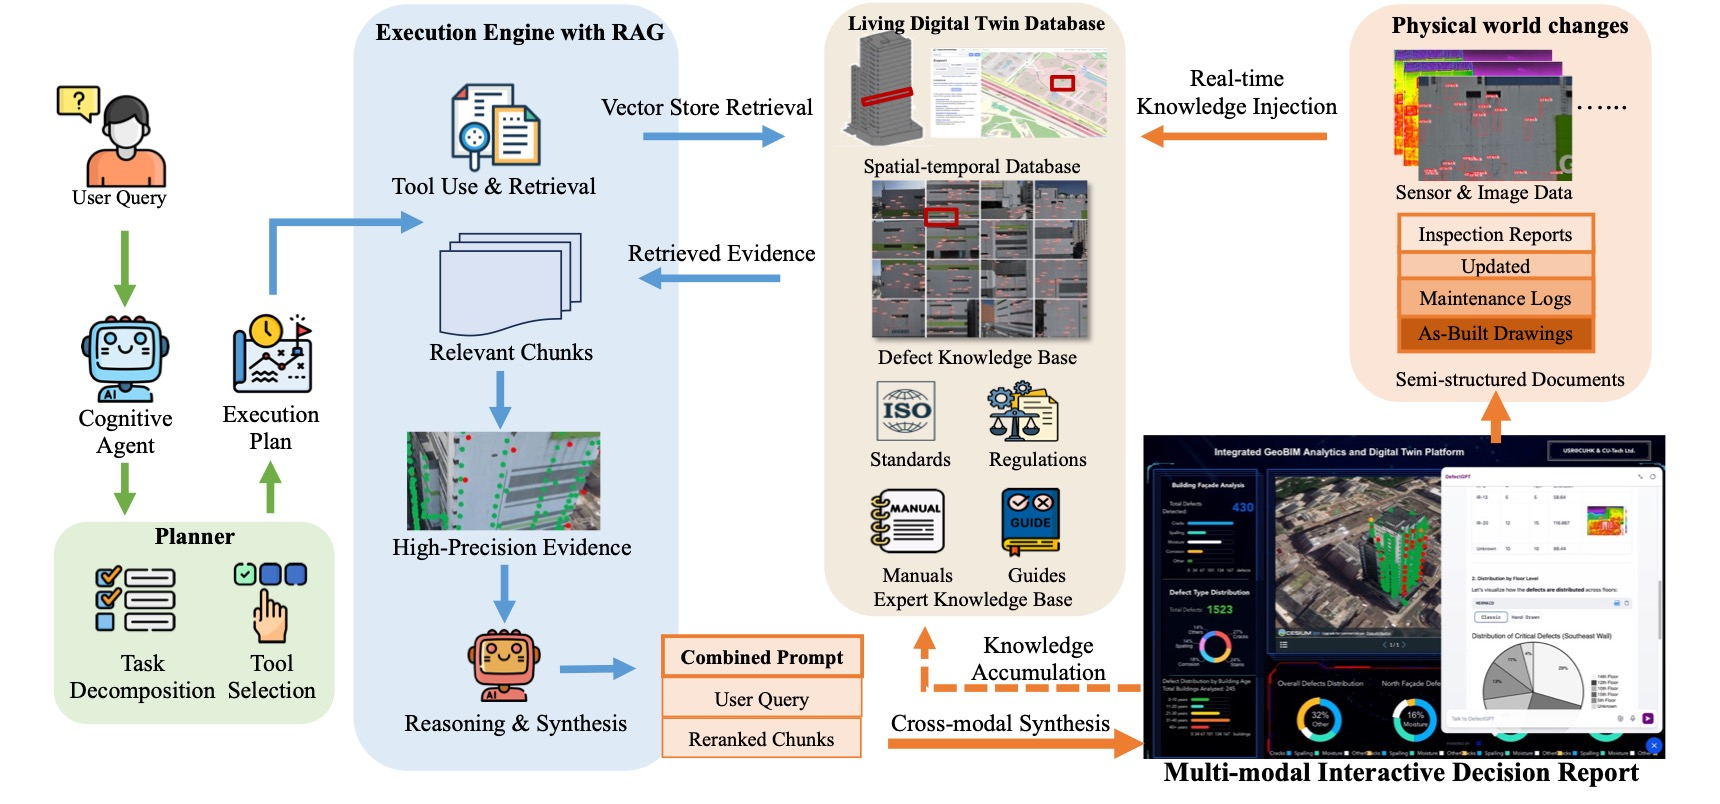
\includegraphics[width=0.9\textwidth]{figures/DefectGPT/cognitive_agent_framework.png}
\caption{The Cognitive Agent Framework showing the plan-retrieve-synthesize architecture with planner for task decomposition, execution engine for tool orchestration, and reasoning \& synthesis for evidence-based generation.}
\label{fig:cognitive-agent-framework}
\end{figure}

\subsection{Planner: Task Decomposition}

The Planner module, corresponding to the left side of Figure~\ref{fig:cognitive-agent-framework}, serves as the strategic intelligence of the system. When receiving a complex user query $Q$, the planner first performs task decomposition. For example, it decomposes the question "Find all high-risk cracks mentioned in reports over the past year on the south facade of Building A, and evaluate their grades according to specifications" into three sub-tasks: (1) locate all components on Building A's south facade; (2) retrieve relevant inspection reports from the past year; (3) find regulatory clauses for crack risk assessment.

The decomposition process follows a formal planning approach:
\begin{equation}
\text{Plan}(Q) = \{t_1, t_2, ..., t_n\} \text{ where } t_i = (\text{action}, \text{parameters}, \text{dependencies})
\end{equation}

Subsequently, the planner performs tool selection, matching optimal retrieval tools for each sub-task. For instance, selecting BIM database APIs for sub-task 1, and vector retrieval tools for sub-tasks 2 and 3. This intelligent routing ensures that each query component is handled by the most appropriate specialized system \cite{yao2022react}.

\subsection{Execution Engine: Hybrid Retrieval}

The Execution Engine, corresponding to the middle section of Figure~\ref{fig:cognitive-agent-framework}, represents our solution to the context window limitation challenge. Traditional RAG systems typically rely on single vector similarity-based retrieval methods, which are severely inadequate when handling multimodal, structured AEC data.

\begin{figure}[htbp]
\centering
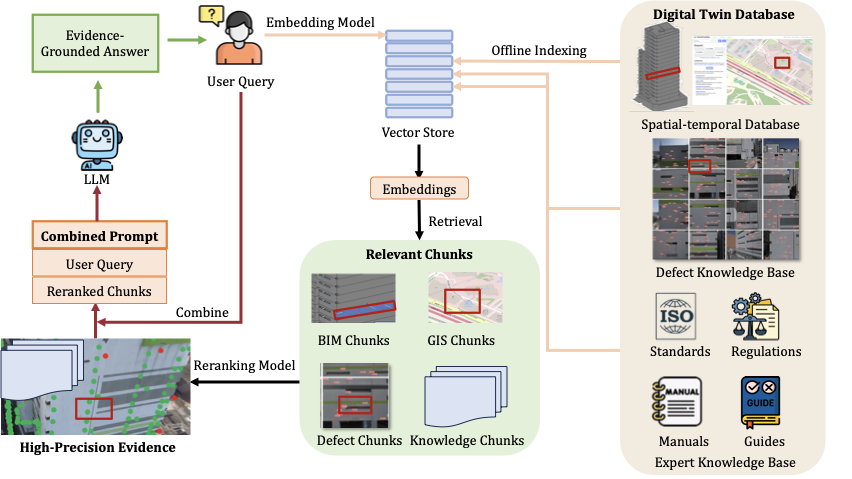
\includegraphics[width=0.9\textwidth]{figures/DefectGPT/hybrid_retrieval_engine.png}
\caption{Hybrid Retrieval Engine architecture demonstrating multi-modal data adapter suite including structured data adapters, time-series adapters, document retrieval adapters, and geometric model adapters, followed by fusion ranking and high-precision evidence extraction.}
\label{fig:hybrid-retrieval-engine}
\end{figure}

Our hybrid retrieval engine, whose workflow is shown in Figure~\ref{fig:hybrid-retrieval-engine}, adopts a more sophisticated and intelligent strategy. Upon receiving a natural language information requirement from the Reasoning Module, the DT-RAG intent analyzer first parses the requirement and decomposes it into multiple sub-tasks. These sub-tasks are then distributed to a parallel suite of specialized data adapters:

\textbf{Structured Data Adapter}: Converts intentions into SQL statements to query asset databases, handling complex joins and aggregations across multiple tables.

\textbf{Time-Series Adapter}: Generates specialized queries to extract sensor readings from time-series databases, including temporal filtering and statistical aggregations.

\textbf{Document Retrieval Adapter}: Utilizes traditional vector retrieval to search for relevant text within unstructured documents using semantic similarity matching.

\textbf{Geometric Model Adapter}: Makes specialized API calls to extract spatial and geometric information from BIM models, including spatial queries and geometric calculations.

The heterogeneous results returned by these parallel queries require sophisticated fusion mechanisms. The most critical step in DT-RAG is integrating these information fragments into a unified, context-rich textual summary through semantic alignment (ensuring information from different sources refers to the same physical entities), temporal synchronization (aligning data from different time periods into coherent temporal narratives), quality weighting (assigning confidence scores based on source reliability and relevance), and contextual summarization (generating natural language summaries optimized for LLM comprehension).

This approach returns heterogeneous results: component IDs, defect data tables, and text segments. A learnable reranking model (typically a Transformer-based Cross-Encoder) then precisely judges "query-evidence pair" relevance, scoring and reordering all initially retrieved information blocks based on their actual contribution to answering the original query.

\subsection{Reasoning \& Synthesis}

The Reasoning \& Synthesis module, corresponding to the bottom section of Figure~\ref{fig:cognitive-agent-framework}, addresses the challenge of factual hallucination through a systematic evidence-driven approach.

\textbf{Evidence Refinement Process}: The evidence refinement process corresponds to the "Reranking" step in our framework. The system performs cross-modal reordering and filtering of initially retrieved relevant chunks, eliminating irrelevant or redundant information to form a high-precision, highly relevant evidence set. This process employs advanced ranking algorithms that consider multiple factors:

\begin{equation}
\text{Score}(d_i, Q) = \alpha \cdot \text{Relevance}(d_i, Q) + \beta \cdot \text{Authority}(d_i) + \gamma \cdot \text{Freshness}(d_i)
\end{equation}

where $d_i$ represents a document chunk, and $\alpha$, $\beta$, $\gamma$ are weighting parameters for relevance, authority, and freshness respectively.

\textbf{Evidence-Driven Generation}: The refined evidence and original user query are combined into a comprehensive prompt that is fed to the LLM. The LLM performs logical reasoning based on evidence in the prompt to generate a final "Evidence-Grounded Answer." This answer not only directly responds to user questions but must include citations to supporting evidence sources.

The generation process is formally constrained as:
\begin{equation}
A = \text{LLM}(Q \oplus E_{refined} \oplus \text{Instructions})
\end{equation}
where $A$ is the generated answer, $Q$ is the query, $E_{refined}$ is the refined evidence set, and $\oplus$ denotes prompt concatenation.

\textbf{Decision Support Visualization}: Generated structured answers are pushed to visualization interfaces in the form of charts, three-dimensional highlights, and interactive dashboards to provide intuitive decision support for users. The system generates comprehensive reports that include executive summary (high-level findings and recommendations), detailed analysis (step-by-step reasoning with evidence citations), visual evidence (interactive 3D models with highlighted defect locations), and actionable recommendations (specific maintenance priorities and procedures).

\section{Experimental Design and Results}

To objectively and quantifiably evaluate DefectGPT architecture effectiveness and specifically respond to research question RQ3, we designed a rigorous controlled comparison experiment. The experiment's core goal is to measure and compare DefectGPT's performance differences with current optimal general methods when completing real-world building diagnosis tasks, and quantify the "Cognitive Gain" brought by our proposed cognitive architecture.

\subsection{Dataset Construction}

We constructed a comprehensive dataset containing real building BIM models, national building code document libraries, and simulated inspection reports and images. The dataset comprises 50 diagnostic query tasks of varying difficulty and complexity, designed in natural language to comprehensively cover typical information needs in building diagnosis scenarios.

\textbf{Task Categories}:
\textbf{Simple Retrieval (15 tasks)}: Single data source information extraction
\textbf{Compound Query (20 tasks)}: Multi-source information fusion requirements  
\textbf{Diagnostic Reasoning (15 tasks)}: Complex analysis, comparison, and evaluation tasks

\textbf{Example Complex Query}: "Please illustrate and explain the vertical distribution pattern of all critical (width > 0.5mm) delamination defects on the southeast facade of Building A, generate a statistical summary table including precise locations, floors, and elevations, and evaluate recommended repair priorities according to the latest 'External Wall Safety Operation Code'."

\subsection{Baseline Model Configuration}

To ensure comparison fairness and persuasiveness, we established two levels of control groups:

\textbf{Naive RAG Baseline}: Represents current standard practice for applying LLMs to knowledge-intensive tasks. All information from the living Digital Twin database is indiscriminately segmented and vectorized into a unified vector database. The system performs one-time cosine similarity-based vector retrieval and feeds results directly to base LLMs.

\textbf{State-of-the-Art LLMs}: Including GPT-4o, Claude 3.5 Sonnet, Mistral-Large-2, Gemini-1.5-Pro, and Llama-3.1-405B, combined with naive RAG baseline to test performance under equivalent (suboptimal) RAG architecture.

Our experimental group (DefectGPT) employs the complete cognitive architecture detailed in Section 4.2, using the same base LLM as control groups to ensure performance differences primarily stem from architectural design rather than base model capability differences.

\subsection{Evaluation Metrics and Results}

We employ a multi-dimensional evaluation metric system to comprehensively measure system performance from different perspectives, including both automated evaluation and human assessment \cite{hernandez2022measuring}.

\begin{figure}[htbp]
\centering
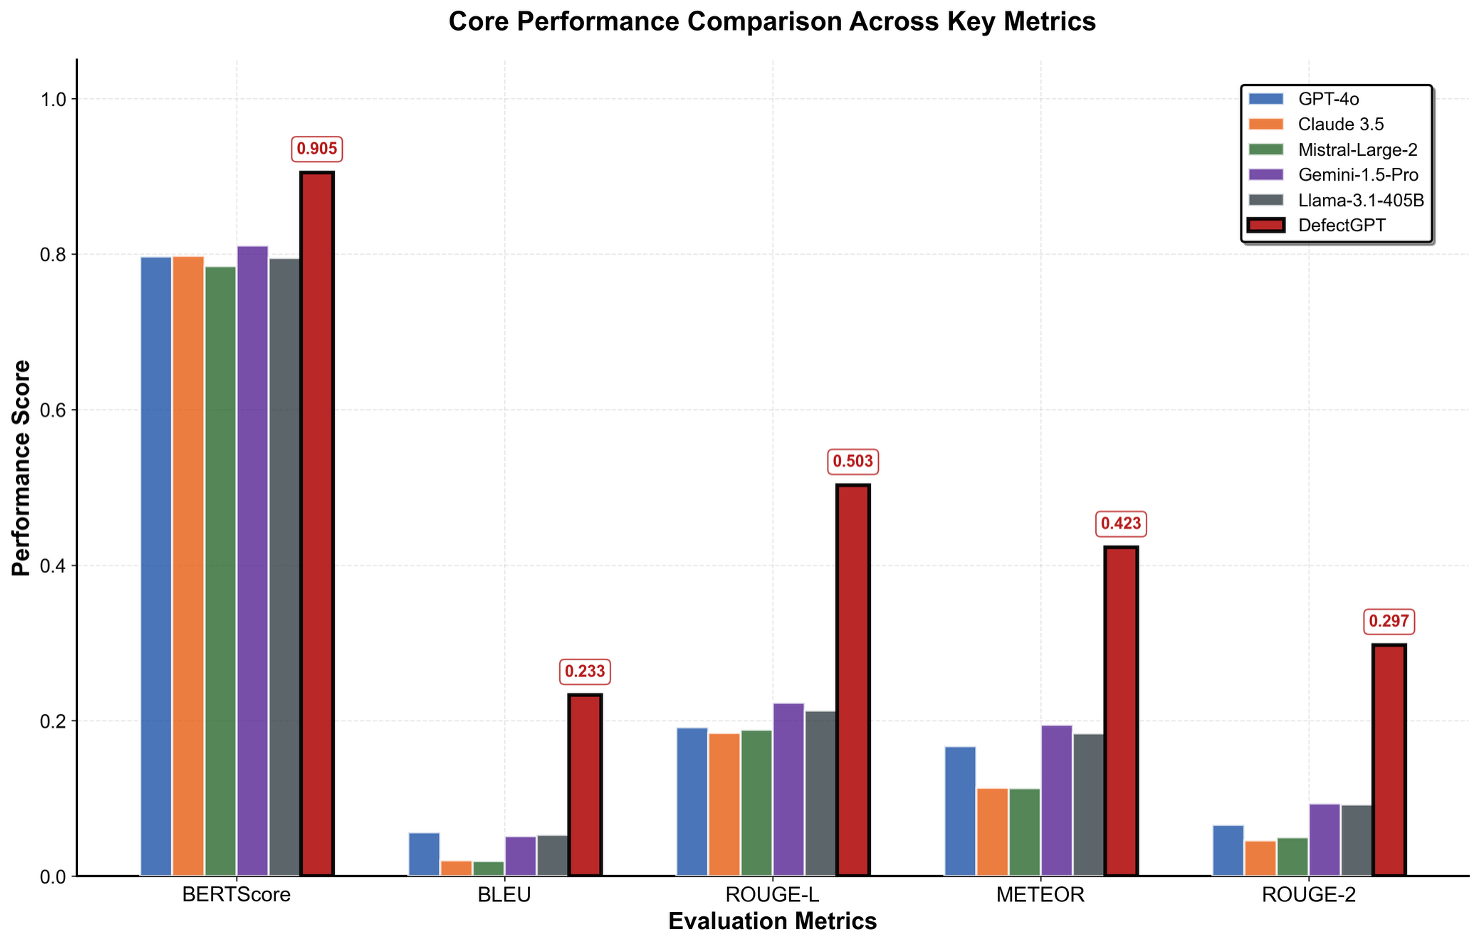
\includegraphics[width=0.9\textwidth]{figures/DefectGPT/performance comparison.png}
\caption{Core Performance Comparison Across Key Metrics showing DefectGPT's superior performance across multiple evaluation metrics (BERTScore, BLEU, ROUGE-L, METEOR, ROUGE-2) compared to state-of-the-art language models. DefectGPT (red bars) demonstrates substantial cognitive gains across all evaluation dimensions.}
\label{fig:performance-comparison}
\end{figure}

Automated evaluation metric comparison results are shown in Figure~\ref{fig:performance-comparison}. This chart summarizes DefectGPT's (represented by red bars) average scores against a series of top-tier general-purpose large language models equipped with naive RAG architecture across five core metrics. The pattern presented by the data is unambiguous: DefectGPT's performance not only leads but achieves breakthrough superiority across every evaluation dimension.

\textbf{BERTScore Performance}: DefectGPT achieved a remarkable average score of 0.905, indicating its generated answers are highly semantically consistent with expert-provided reference answers. In comparison, the best-performing control group model scored only approximately 0.81, representing an 11.7% performance improvement for DefectGPT.

\textbf{ROUGE-L Analysis}: Performance gaps are particularly dramatic in ROUGE-L metrics, which emphasize long sequence coherence and key information completeness—precisely what complex diagnostic tasks require. DefectGPT scored 0.503 while the second-best Llama-3.1-405B scored only 0.22, representing a cognitive gain of 128.6%.

\textbf{Human Expert Evaluation Results}: In blind evaluation by three experts, DefectGPT achieved average scores of 4.8, 4.7, and 4.6 (out of 5) in factual accuracy, completeness, and utility dimensions respectively. In contrast, the best-performing control group model averaged only 3.2, 3.5, and 3.1.


\section{Summary of Findings}

This chapter has successfully demonstrated and validated CORTEX cognitive architecture's exceptional capabilities in handling L1-tier descriptive Digital Twin tasks through systematic study of a real-world building defect diagnosis case. We detailed DefectGPT's design and implementation, where the system's three core engines—hybrid retrieval engine, dynamic knowledge engine, and cognitive agent framework—successfully overcome fundamental challenges of context limitations, knowledge grounding deficits, and factual hallucinations encountered when directly applying large language models to engineering domains.

\subsection{Response to Research Questions}

This chapter's work systematically demonstrates how instantiating a "Living Brain" prototype, as shown on the right side of the Dynamic Knowledge Engine concept, provides a concrete implementation solution for RQ1. By constructing a three-tier Digital Twin framework specifically oriented toward AI decision-making needs rather than engineering implementation metrics, we successfully created a standardized "capability testing ground" that enables systematic evaluation of cognitive architectures across different complexity levels.

The experimental results validate how DefectGPT's perception module effectively handles complex diagnostic tasks, responding to RQ2. Through the plan-retrieve-synthesize architecture, we successfully bridged the cognitive-physical gap by enabling LLMs to operate on evidence-based reasoning rather than hallucination-prone speculation. The substantial cognitive gains measured across multiple metrics provide quantitative evidence for RQ3, demonstrating that sophisticated architectural design can significantly enhance AI system performance in knowledge-intensive domains.

\subsection{Architectural Innovations}

The DefectGPT implementation reveals several key insights about integrating LLMs with structured knowledge systems:

\textbf{Evidence-First Principle}: By mandating that all reasoning be grounded in retrievable evidence, we eliminated the primary source of factual hallucinations while maintaining the flexibility and interpretability that make LLMs attractive for human-AI interaction.

\textbf{Multimodal Integration Strategy}: The hybrid retrieval engine demonstrates that effective integration of structured, temporal, and textual data requires specialized adapters rather than naive vectorization approaches.

\textbf{Dynamic Knowledge Management}: Real-time knowledge injection proves superior to periodic retraining for maintaining system currency with evolving physical world conditions.

\subsection{Limitations and Future Directions}

Current implementation limitations include dependency on data schema standardization, challenges in real-time data stream processing, and computational overhead of the multi-engine architecture. Future research directions include investigation of federated learning approaches for distributed knowledge management, development of more sophisticated causal reasoning mechanisms, and exploration of active learning strategies for continuous system improvement.

Rigorous quantitative and qualitative experimental analysis consistently shows that our proposed architecture significantly outperforms current optimal general RAG methods. The substantial "cognitive gains" calculated and the deep reasoning and multimodal interaction capabilities demonstrated in specific cases powerfully prove our core argument: for knowledge-intensive, logically rigorous, and safety-critical professional domains, a carefully designed, evidence-centered cognitive architecture is key to achieving reliable artificial intelligence applications.
